A continuación mostramos un pairplot de las variables.

\begin{figure}[H]
    \centering
    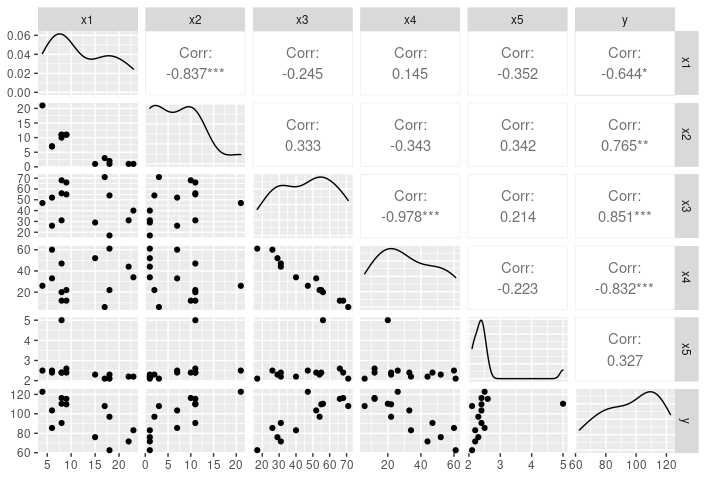
\includegraphics[width=1\textwidth]{resources/GGPairs.png}
    \caption{Pair Plot de las variables}
\end{figure}

\subsubsection*{Análisis general de coeficientes}
En el siguiente gráfico podremos ver con mayor facilidad los coeficientes que dieron significativamente altos entre las covariables. 

\begin{figure}[H]
    \centering
    
\includegraphics[width=0.8\textwidth]{resources/HeatMapRho.png}
    \caption{Se observa que algunas variables presentan un alto coeficiente de correlación.}
\end{figure}
Los coeficientes entre las covariables y la variable a predecir se verán más adelante.
\vskip0.2cm\textbf{X3 vs X4}\\
Lo primero que destacamos del gráfico es la correlación entre las variables $X_{3}$ y $X_{4}$, dado que se acerca mucho a -1 ($\hat{\rho}_{_{X_{3},X_{4}}} = -0.978$). Esto se corresponde con el gráfico de dispersión entre estas variables, cuyo gráfico se encuentra en la parte inferior de la matriz, y destacamos a continuación.

\begin{figure}[H]
    \centering
    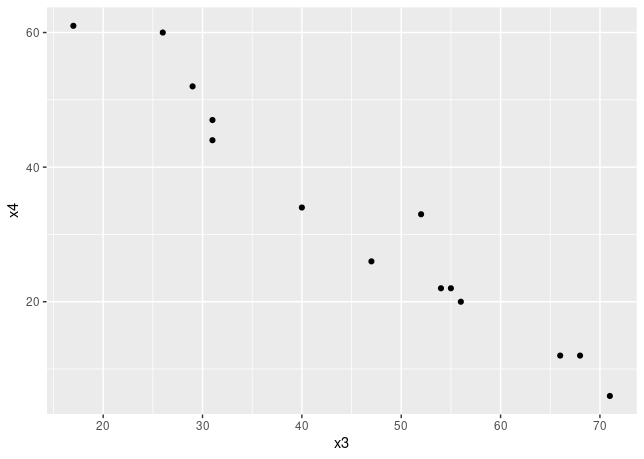
\includegraphics[width=0.8\textwidth]{resources/X3vsX4.png}
    \caption{Gráfico de dispersión entre x3 y x4}
\end{figure}

Viendo este gráfico podemos observar que a medida que aumenta $X_3$, tiende a disminuir $X_4$.\\
Esto nos informa que parece haber una relación lineal muy fuerte entre las variables $X_3$ y $X_4$, situación que habrá que tener en cuenta a la hora de realizar la regresión lineal sobre la variable objetivo ($Y$).
Asimismo, además, podemos observar en el gráfico que las correlaciones entre las diferentes variables con $X_3$ y con $X_4$, en modulo, se parecen.
Por ejemplo, $\hat{\rho}_{_{X_{3},Y}} = 0.851$ y $\hat{\rho}_{_{X_{4},Y}} = -0.832$

\subsubsection*{Valores atípicos}
Pudimos advertir la presencia de valores atípicos en los datos observando sobretodo la fila de la variable $X_5$ y la columna de la variable $X_2$ cuyos valores representaremos en el siguiente gráfico con un boxplot:

\begin{figure}[H]
    \centering
    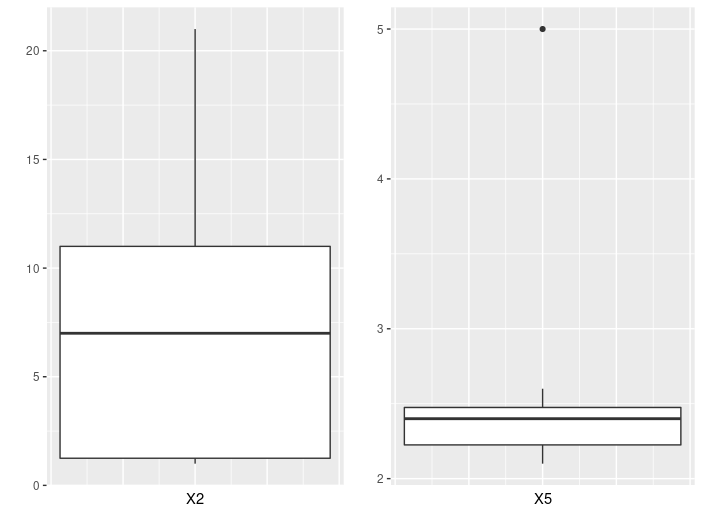
\includegraphics[width=0.6\textwidth]{resources/boxplots_X2_X5.png}
    \label{fig:my_label}
\end{figure}

Desde ya, no podemos descartar estos puntos a pesar de que sean valores atípicos. Sin embargo, debemos prestarles especial atención a la hora de analizar la muestra y más aún al generar nuestro modelo.

\subsubsection*{Relación con la variable objetivo}

\begin{figure}[H]
    \centering
    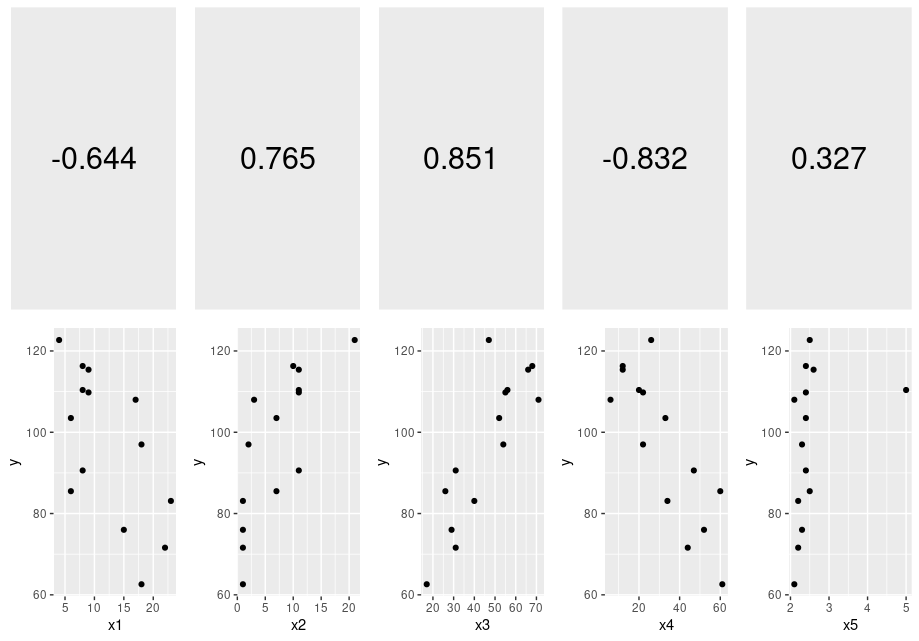
\includegraphics[width=1\textwidth]{resources/x_vs_y.png}
    \caption{Relación entre las variables x y la variable y}
\end{figure}

Podemos ver que a priori, las variables con mayor coeficiente de correlación con Y son X2, X3 y X4 siendo estas dos últimas las de mayor coeficiente.\\
Esto nos servirá como una primera impresión sobre cuáles variables tendrán, a priori, un impacto sobre la variable objetivo.\\
\textbf{Obs:} vemos por ejemplo que la variable X5 tiene un coeficiente de correlación muy bajo, pero cabe destacar que presenta un valor atípico que podría estar provocando que obtengamos una idea errónea sobre su impacto.
